\section{Experimental Evaluation: Parallel Validator Reordering}
\label{sec:experiments:parallel}

\begin{figure*}
	\centering
	\begin{minipage}[b]{0.31\linewidth}
		\centering
		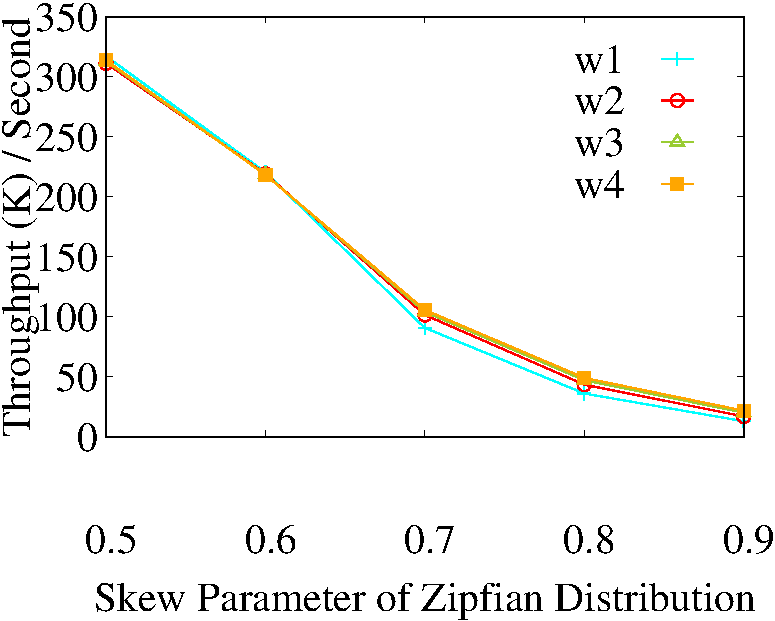
\includegraphics[width=\textwidth]{./exp_fig/reorder/tps}
		%	\vspace{-2em}
		\caption{Throughput varying the number of reordering workers}
		\label{fig:reorder:tps}
	\end{minipage}    
	\begin{minipage}[b]{0.31\linewidth}
		\centering
		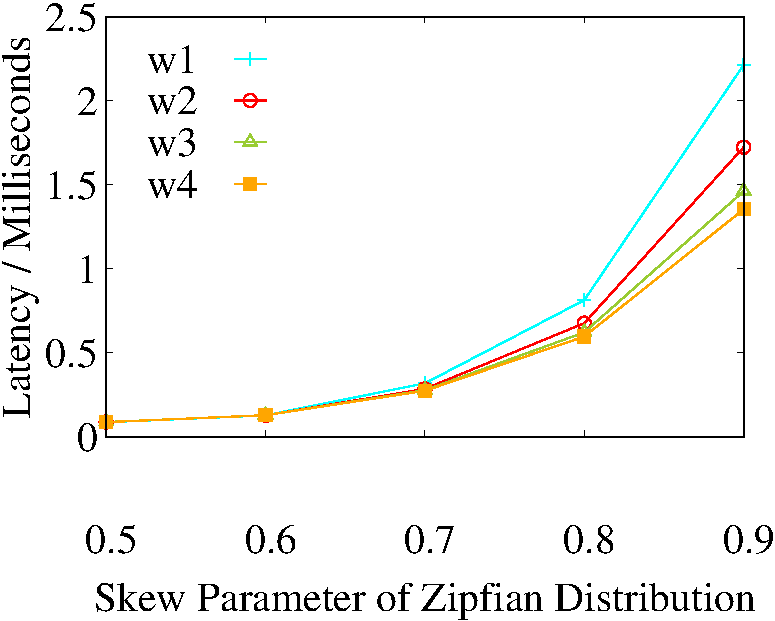
\includegraphics[width=\textwidth]{./exp_fig/reorder/latency}
		%	\vspace{-2em}
		\caption{Average latency varying the number of reordering workers}
		\label{fig:reorder:latency}
	\end{minipage}    
	\begin{minipage}[b]{0.31\linewidth}
		\centering
		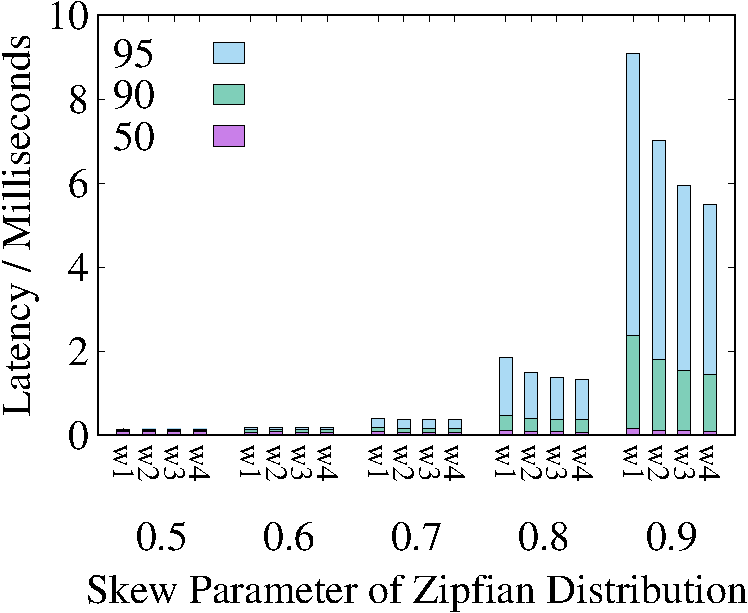
\includegraphics[width=\textwidth]{./exp_fig/reorder/percent95_latency}
		%	\vspace{-2em}
		\caption{Percentile latency varying the number of reordering workers}
		\label{fig:reorder:p95}
	\end{minipage}    
	%    \begin{minipage}[b]{0.31\linewidth}
	%	\centering
	%	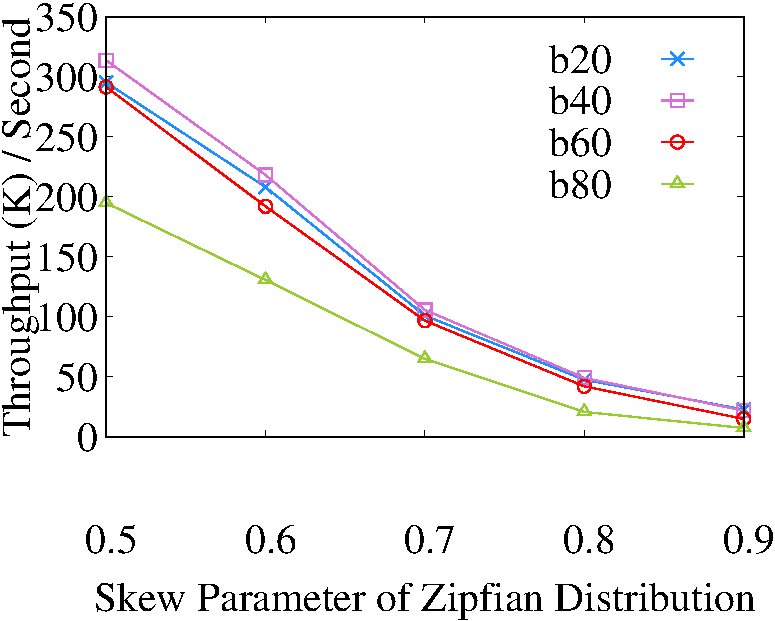
\includegraphics[width=\textwidth]{./exp_fig/bsize/tps}
	%	\vspace{-2em}
	%	\caption{Throughput with various batch sizes}
	%	\label{fig:bsize:tps}
	%	\end{minipage}    
	%    \vspace{-1em}
\end{figure*}


We evaluate the benefit of parallelism in the validator. Since we have observed that the reordering of FVS is the most time consuming subcomponent in the validator, we increase the number of threads to parallelize batch reordering as described in Appendix~\ref{sec:parallel}. 
Figure~\ref{fig:reorder:tps} and~\ref{fig:reorder:latency} show the throughput
and the average latency with the number of reordering workers from $1$ to $4$
($w1$, $w2$, $w3$, $w4$). The performance improves significantly with more reordering workers when data skew is medium to high. With $4$ workers, the throughput increases by up to $2.6\times$, and the average latency reduces by up to $39\%$, as compared to the result with $1$ worker. Figure~\ref{fig:reorder:p95} shows the percentile transaction latency. With more reordering workers, more transactions are reordered concurrently, and the transaction queuing time at validator is reduced. With $4$ workers, the tail latency reduces by up to $41\%$.\eat{ The improvement is not linear since the bottleneck of the system shifts to other
components as we increase the capacity of reordering.}

%The system can further scale up once the capacity of other components is carefully engineered and scaled, which is out of scope for this paper.
\eat{
In summary, parallel reordering reduces the queuing time for transactions, which leads to better throughput, average latency, and percentile latencies. Since 3 reordering workers have provided most of the benefit of parallel reordering in our configuration, we set the number of reordering workers to 3 in the reminder of our experiments.}
